\chapter{绪论}
\section{研究背景}
随着机器人技术不断向非结构化、复杂化和极端环境拓展，机器人系统正面临由单一结构化任务向复杂环境自助作业任务的转变。传统刚性机器人通常具有较高的定位精度、负载能力和控制稳定性，适用于结构化工业场景中的重复性操作任务。然而，在狭窄空间、复杂曲面、柔顺接触环境以及水下等弱视觉或无视觉场景中，传统刚性机器人往往难以同时满足高灵活性、高适应度和安全交互的要求。尤其在管道检测、水下作业、柔性抓取和复杂环境探测等任务中，机器人不仅需要具备一定的结构支撑能力和任务执行能力，还需要具备对环境变化和自身形态变化的适应能力。因此，发展兼具柔顺性、可控性和环境适应能力的新型连续体机器人系统，已成为机器人领域的重要研究方向之一。

连续体机器人可以实现连续弯曲、柔顺变形和多自由度运动，相较于传统离散关节机器人，其能够在复杂空间中表现出更高的运动灵活性和环境适应性。然而，完全柔性的结构虽然具有良好的变形能力，但在承载能力、形态保持、传感器集成和运动控制等方面仍然存在一定的限制。相比之下，刚柔耦合的连续体结构通过在柔性结构中引入刚性节点、模块化单元或阵列化支撑形式，能够保持一定柔顺变形能力的同时，引入一定的空间约束条件，也能提高结构稳定性和可控性。这类结构既不同于传统刚性连杆机构，也不同于完全柔性的软体机器人，而是一种兼具刚性约束和柔性变形特征的复杂连续体系统。其在复杂环境感知、柔顺操作、空间形态重构中具有独特的优势，也具有广阔的应用前景。

然而，刚柔耦合连续体结构的复杂变形特性也给机器人自身状态感知带来了全新的挑战。与传统刚性机器人可以通过关节编码器直接获取关节角度不同，刚柔耦合连续体的运动状态通常表现为多个节点姿态、局部应变、整体弯曲形态和空间构型之间的耦合变化，在多种载荷约束在可能产生弯曲、扭转、拉伸等多种耦合变化，使得机器人自身形态难以通过单一测量量直接描述。如果缺乏准确的自感知能力，对机器人进行下游的闭环控制、形态重建或者环境互动等复杂任务会造成巨大的影响。因此自感知技术已经成为刚柔耦合连续体结构由结构设计走向实际应用的关键基础。

自感知是指机器人依靠自身集成的传感系统获取其姿态、变形、运动和接触状态等信息的能力。对于刚柔耦合连续体结构而言，自感知不仅需要或者局部节点的姿态变化，还需要反映结构整体的三维形态、局部弯曲以及外部作用下的变形响应。在封闭空间、水下环境或遮挡严重的场景中，外部视觉系统往往受到视场、光照、浑浊度和安装条件限制，难以持续提供可靠的机器人形态信息。此时，机器人必须更多依赖自身传感系统实现状态估计，从而支撑后续的运动控制、抓取操作和环境交互。
目前，用于连续体机器人和柔性结构状态感知的方法主要包括视觉测量、磁定位、光纤传感、柔性应变传感、惯性测量等\cite{Chen2024VisionbasedTF,Yao2025FastAdaptivePP}。外部视觉方法能够提供较直观的空间位姿信息，但对观测条件依赖较强，特别在遮挡、封闭或水下环境中应用受到极大限制。光纤传感具有灵敏度高、抗电磁干扰能力强等优点，但其布设和封装工艺复杂，对系统集成和信号解耦要求高。应变传感器能够直接反映结构局部变形，适合用于柔性或者刚柔耦合结构的弯曲感知，但其测量结果易受到材料非线性、迟滞和温度变化等因素影响。惯性测量单元（Inertial Measurement Unit, IMU）具有体积小、响应快、易集成等优势，能够提供短期内较准确的局部姿态和动态运动信息，但单独使用时存在误差累积和漂移问题。因此单一的传感方式往往难以满足刚柔耦合连续体在三维形态估计、长期稳定感知和复杂环境适应方面的需求。

分布式多模态传感为刚柔耦合连续体结构自感知提供了新的技术路径，通过在结构关键点布设多类型传感单元，可以同时获取局部姿态、动态响应和结构应变等多维信息。节点化布设方式有助于将连续体的复杂整体形态转化为若干局部状态的组合表征，多模态测量方式则能够利用不同传感信息之间的互补关系，提高状态估计的准确性、稳定性和鲁棒性。相比依赖外部观测系统的感知方法，内嵌式或随体式传感阵列能够随结构一起进入复杂环境，在遮挡、封闭、水下等外部观测受限条件下持续获取自身状态信息，因此更适合服务于复杂环境中的机器人操作和结构状态估计任务。

近年来刚柔耦合连续体结构已经取得了显著进展，但其在实际应用中的自感知任务仍面临诸多挑战：（1）传感单元长期稳定性和可靠性问题：分布式传感器虽然精度高，但在长期使用中可能受到环境因素、材料疲劳和自身漂移等因素影响，导致测量精度下降从而影响整体状态估计的可靠性；（2）刚性传感器与柔性结构的耦合问题：传感器的安装和封装形式可能会对柔性结构的变形特征产生影响，大量刚性传感器可以增加传感阵列的约束条件降低求解难度，但也可能改变结构的柔顺性和变形模式；（3）多模态信息融合与状态估计难题：目前针对刚柔耦合连续体结构的状态估计方法主要依赖于单一传感器，缺乏针对多模态传感信息的融合方法，如何有效利用不同传感器之间的互补信息，实现对复杂变形状态的准确估计仍然是一个亟待解决的关键问题。

针对上述问题，本文聚焦刚柔耦合连续体结构的分布式多模态自感知与三维形态估计方法研究，通过理论建模、算法优化、实验验证与系统集成的递进式研究，突破了刚柔耦合连续体结构自感知的关键技术瓶颈，旨在为刚柔耦合连续体结构的自主感知、运动控制和环境交互提供理论基础和技术支撑，推动其在复杂环境中的应用发展。
\section{国内外研究现状}
\subsection{基于多传感融合的三维形态估计方法}
连续体结构和软体结构通常具有连续变形能力，其空间状态不能简单地由有限个离散关节变量描述。对于刚柔耦合连续体结构而言，刚性节点、柔性连接和外部接触之间存在耦合关系，结构形态往往表现为节点姿态、局部应变、整体曲率以及空间中心线的综合变化。因此，三维形态估计不仅是连续体结构运动控制的基础问题，也是刚柔耦合传感阵列实现自感知的核心问题。近年来，连续体结构感知研究已经从单一传感器测量逐渐转向多源感知融合。

早期连三维形态估计方法多基于几何假设模型或单一传感信息，常见的有分段常曲率假设、分段多项式曲率模型、Cosserat杆理论、Frenet-Serret框架以及有限元模型等。这类方法能够在一定程度上将结构变形转化为中心线重建问题，并且具有良好的物理解释性。然而连续体结构在实际运行中常常受到重力、驱动误差、材料非线性和外部载荷的影响，其变形往往并不能满足理想常曲率假设。Armanini等在研究中指出软体和连续体机器人建模已经形成多种理论路线，但不同模型对结构参数、边界条件和数值计算的依赖差异很大，单一模型难以在所有工况下保持稳定精度\cite{armanini2023soft}。因此，越来越多的研究开始将传感信息、几何约束和数据驱动模型结合起来，以提高三维形态估计的适用性。

现有研究中，多源融合三维形态估计主要形成了三类技术路线。第一类是外部观测与内嵌传感融合，即利用视觉、荧光透视、电磁定位或者医学影像等外部观测手段获取全局空间约束，同时利用FBG、柔性应变或其他内嵌式传感器获取局部变形信息。视觉或影像信息能够提供结构在全局坐标系中的位置或轮廓，但受外界条件影响较大，内嵌式应变或光纤传感能够反映结构本身弯曲状态，但存在坐标漂移、积分误差和局部约束不足等问题。因此两类信息融合可以一定程度上兼顾全局观测和本体感知。Wang等将眼在手视觉信息与单芯FBG的稀疏应变数据融合，用于连续体机器人的位姿估计与控制，如图~\ref{Fig_Research_Status_1_1}(a)所示。该方法针对图像特征不足时视觉估计不稳定的问题引入了应变信息作为补充，使连续体机器人在视觉退化条件下仍能保持较好的位姿估计能力\cite{wang2023learning}。Ha等将电磁跟踪传感器与多芯光纤形状传感结合，用于导管三维形态重建，并提出了同轴导管跟踪融合框架，如图~\ref{Fig_Research_Status_1_1}(b)所示，说明全局定位传感器可以有效弥补光线形状传感在末端误差与全局坐标对齐的不足\cite{ha2023sensor,ha2023fusion}。Lawson等提出基于双平面荧光透视和定制不透射线标记的导管形状和姿态估计方法，实现了对微导管的形状与滚转角估计\cite{lawson2025fluoroscopic}，如图~\ref{Fig_Research_Status_1_1}(c)所示。Yi 等提出基于 FBG 传感阵列和双目视觉的智能结肠镜三维形状显示方法\cite{shi2016shape}，其实验系统如图~\ref{Fig_Research_Status_1_1}(d)所示，将 FBG 阵列用于感知结肠镜插入段形状，并利用双目视觉定位手柄位姿，从而实现器械空间形态的显示。这类研究表明，外部观测手段和内嵌传感数据融合可以显著提高形状估计精度，但其适用性仍依赖外部观测设备和稳定标定关系，在面向水下、封闭或者无视觉环境中该类方法更多适合作为标定和对照手段，而难以作为长期自主感知的唯一方案。
\begin{figure}[!htbp]
    \centering
    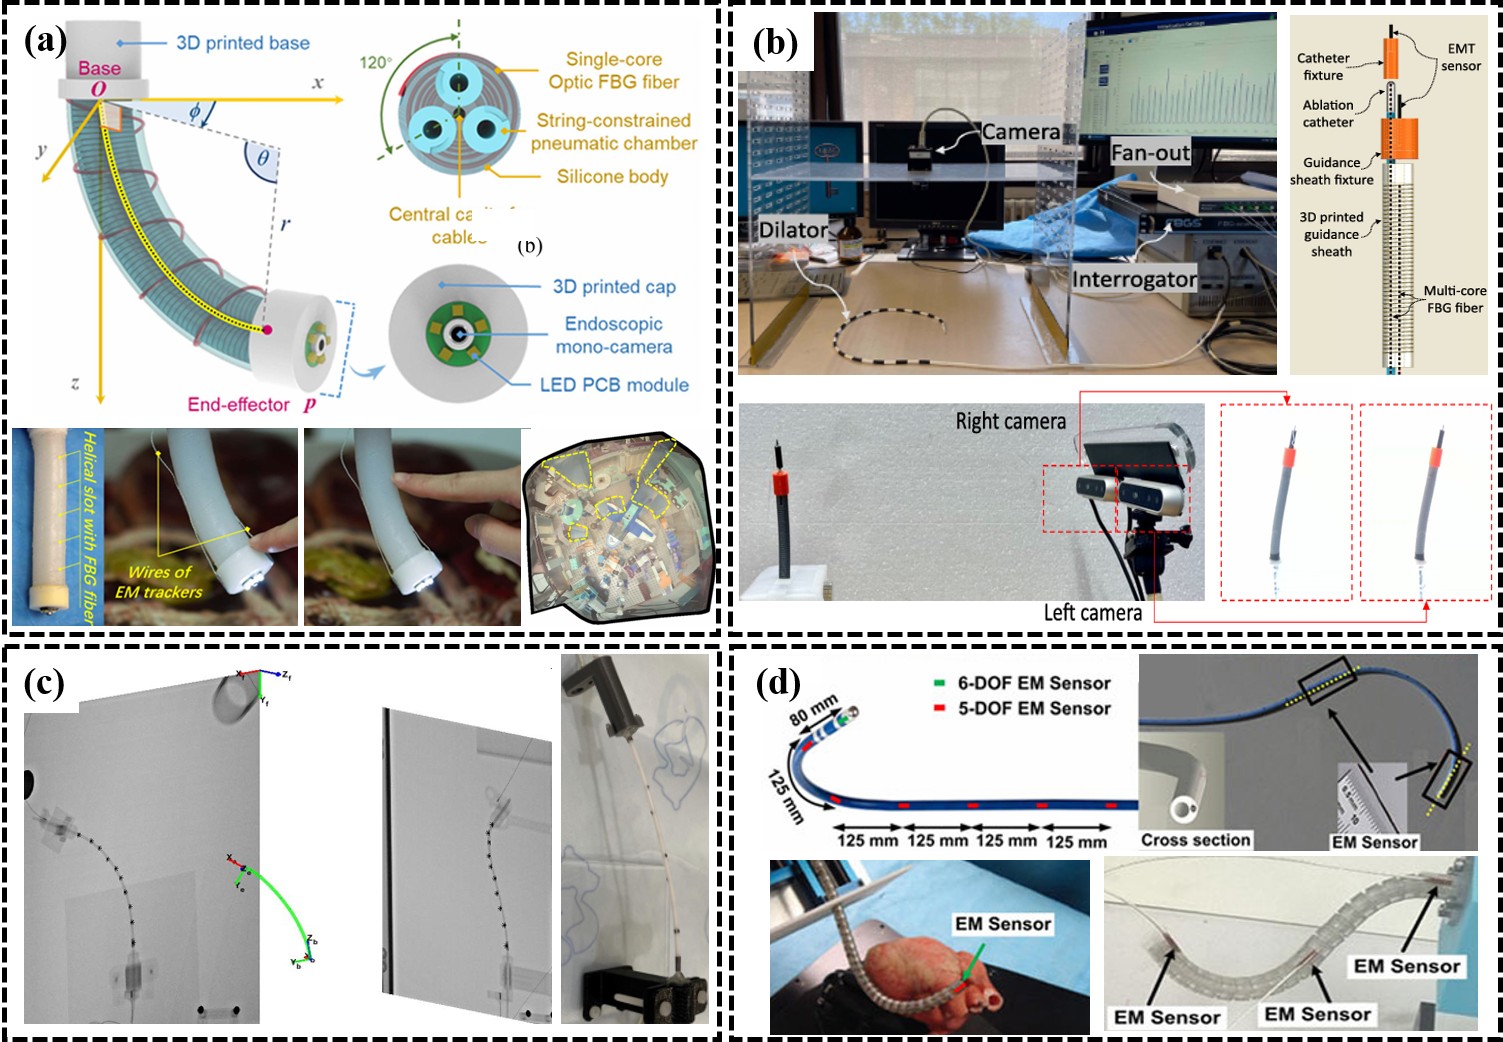
\includegraphics[width=0.88\linewidth]{figure/chapter1/Fig_Research_Status_1_1.png}
    \caption{外部观测与内嵌传感融合的连续体结构三维形态估计研究示例：
（a）光纤光栅与视觉信息融合的软体连续体结构形态感知；
（b）视觉观测与光纤形状传感融合的导管形态重建；
（c）双平面荧光透视下的导管三维形状与姿态估计；
（d）电磁跟踪与多芯光纤形状传感融合的导管空间形态重建。}
    \label{Fig_Research_Status_1_1}
\end{figure}
\FloatBarrier

第二类方法是基于应变、曲率信息与模型约束的形态估计方法。该类方法不完全依赖外部视觉，而是利用结构内部的应变、曲率或者节点位姿信息，结合运动模型重建整体形态。Liu 等提出基于稀疏分布柔性应变传感器的三维形态重建方法，如图~\ref{Fig_Research_Status_1_2}(a)所示。该方法将小型可拉伸电容应变传感器布设在软体结构表面，并将测量应变输入带力学约束的优化框架，从而实现软体杆、软体抓手和复杂软体结构的形态重建\cite{liu2025modelbased}。Hou 等提出将 FBG 传感数据与运动学模型结合实现连续体机器人形态感知，如图~\ref{Fig_Research_Status_1_2}(c)所示。该方法通过自适应加权粒子滤波融合模型预测和 FBG 测量，降低了单独依赖模型或光纤传感带来的误差\cite{hou2025sensing}。Lu 等将多芯 FBG 本体感知与在线学习方法结合，用于非结构化环境下连续体和软体机器人的三维形态伺服，如图~\ref{Fig_Research_Status_1_2}(b)所示。该方法利用数据驱动补偿降低模型误差和传感器漂移对形态估计的影响\cite{lu2024adaptive}。Shen 等针对绳驱动连续体机器人提出基于可拉伸电容传感器的形状感知与运动学控制方法，如图~\ref{Fig_Research_Status_1_2}(d)所示。该方法通过柔性骨架表面布设的可拉伸电容传感器测量弯曲变形，并结合几何建模计算连续体关节变量\cite{shen2024shape}。
\begin{figure}[!htbp]
    \centering
    
\includegraphics[width=0.88\linewidth]{chapter1/Fig_Research_Status_1_2_zh.png}
    \caption[基于应变、曲率信息与模型约束的连续体结构形态估计方法示例]{
    基于应变、曲率信息与模型约束的连续体结构形态估计方法示例：
    （a）稀疏分布柔性应变传感器与力学约束优化结合的软体结构形态重建；
    （b）多芯 FBG 本体感知与在线学习结合的连续体和软体机器人三维形态伺服；
    （c）FBG 传感数据与运动学模型融合的连续体机器人形态感知；
    （d）可拉伸电容传感器与几何模型结合的绳驱动连续体机器人形状感知。}
    \label{Fig_Research_Status_1_2}
\end{figure}
\FloatBarrier

第三类方法是基于节点姿态信息与多模态约束的形态估计方法。该类方法以惯性测量单元、姿态传感器或离散位姿测量为主要信息来源，通过多个节点的姿态约束重建连续体结构的空间形态。与应变传感器相比，IMU 能够直接提供局部姿态和动态响应信息；与外部视觉相比，IMU 不依赖观测视线，适合布设在连续体结构或刚柔耦合结构的关键节点上。然而，IMU 单独使用时容易受到陀螺仪漂移、磁干扰、安装方向误差和局部柔性变形不可观测等因素影响，因此通常需要与应变、几何模型或运动学约束进行融合。An等提出了一种融合局部应变和离散位姿的软连续体机器人形态重建方法，通过 FBG 提供局部弯曲曲率约束，再利用 IMU 提供的姿态信息修正仅依靠应变积分产生的空间累积误差，该方法解决了传统曲率积分方法中误差沿弧长累积的问题\cite{an2024shape}。Stella等将IMU姿态估计与分段常曲率运动学约束结合，用PCC模型对IMU形态估计中的漂移进行滤波处理，从而延长软体机器人基于IMU的形态测量时间并提高估计稳定性\cite{stella2023soft}。Peng 等在 2024 年提出一种基于多个 IMU 的绳驱动连续体机械臂鲁棒形状估计方法\cite{peng2024tendon}，通过多节点姿态信息重建连续体结构形态，说明多 IMU 阵列可以为连续体结构提供较强的空间方向约束。Meng 等提出弹簧—IMU 融合本体感知方法，将电感弹簧提供的几何变形信息与 IMU 提供的姿态信息结合，并用于软体机械臂反馈控制\cite{meng2024spring}；该研究表明，几何传感与惯性传感在大伸长、大弯曲结构中具有明显互补性。国内许立松等在 2025 年提出基于切向量拟合的连续体机械臂多 IMU 形态估计算法\cite{xu2025multiimu}，基于 Cosserat 杆理论描述连续体机械臂形变，以减弱传统分段常曲率假设在复杂形态下的局限。相关研究如图~\ref{fig:research_status_1_3} 所示。
\begin{figure}[!htbp]
    \centering
    
\includegraphics[width=\textwidth]{chapter1/Fig_Research_Status_1_3.png}
    \caption{基于节点姿态信息与多模态约束的连续体结构形态估计方法研究现状：
    (a) 融合 FBG 局部应变与 IMU 离散姿态信息的软连续体机器人形态重建方法\cite{an2024shape}；
    (b) 结合 IMU 姿态估计与分段常曲率运动学约束的软体机器人形态估计方法\cite{stella2023soft}；
    (c) 基于多 IMU 阵列的绳驱动连续体机械臂鲁棒形状估计方法\cite{peng2024tendon}；
    (d) 弹簧--IMU 融合本体感知方法及其在软体机械臂反馈控制中的应用\cite{meng2024spring}；
    (e) 基于切向量拟合与 Cosserat 杆理论的连续体机械臂多 IMU 形态估计算法\cite{xu2025multiimu}。}
    \label{fig:research_status_1_3}
\end{figure}

除上述路线外，近年来还出现了基于新型传感材料和学习模型的三维形态估计方法，Baaij等使用多个磁传感器学习连续体软体结构的三维本体感知，利用神经网络处理磁场测量与机器人形态之间的非线性关系\cite{baaij2023learning}。Shah等提出利用可拉伸形状感知片将液态金属电路和方向传感相结合，用于对柔性片状结构和软体表面的形状进行估计\cite{shah2023stretchable}。Del Bono等提出集成软光波导的微型软连续体机器人\cite{delbono2024soft}，通过功能化医用软管实现三维光学形状感知，为小尺度柔性结构中的低成本光学传感提供了新的方案。Zhan 等在 2025 年提出物理信息神经位姿估计方法，将物理约束引入神经网络以实现软连续体机器人的实时形态重建\cite{zhan2025physics}。Alian进一步将电阻抗断层成像与神经网络结合，提出面向软连续体内窥机器人的可扩展三维形态感知方法，并在离体猪结肠环境中进行了验证\cite{alian2026electrical}。上述基于新型传感材料和学习模型的代表性研究如图~\ref{fig:research_status_1_4} 所示。新型传感材料和学习算法提高了复杂非线性形态估计能力，但也带来了数据需求、泛化能力、可解释性和长期可靠性等问题。
\begin{figure}[!htbp]
    \centering
    
\includegraphics[width=0.88\textwidth]{chapter1/Fig_Research_Status_1_4.png}
    \caption[基于新型传感材料和学习模型的三维形态估计方法研究现状]{基于新型传感材料和学习模型的三维形态估计方法研究现状：
    (a) 基于多磁传感器与神经网络的连续体软体结构三维本体感知方法\cite{baaij2023learning}；
    (b) 基于可拉伸形状感知片的柔性片状结构和软体表面形状估计方法\cite{shah2023stretchable}；
    (c) 集成软光波导的微型软连续体机器人三维光学形状感知方法\cite{delbono2024soft}；
    (d) 面向软连续体机器人的物理信息神经位姿估计方法\cite{zhan2025physics}；
    (e) 结合电阻抗断层成像与神经网络的软连续体内窥机器人三维形态感知方法\cite{alian2026electrical}。}
    \label{fig:research_status_1_4}
\end{figure}

总体来看，连续体结构三维形态估计已经行程了从外部观测到内部感知，从单一传感到多源融合，从解析模型到数据驱动与物理约束结合的发展趋势。外部视觉、荧光透视和电磁定位等方法能够提供全局空间信息，但其工作条件受到环境限制。光纤和柔性应变传感器能够提供局部变形信息，但其长期稳定性和局部整体映射仍存在难点。IMU能够提供节点姿态和动态响应，适合刚柔耦合结构的节点化布设，但单独使用时难以完整表征连续变形。而模型约束和数据驱动方法能够显著提升估计能力，但其依赖稳定的训练数据以及大量的标定工作。

面向刚柔耦合连续体结构传感阵列而言，现有的研究仍然存在三个方面明显的不足：（1）大部分方法仍依赖视觉或外部定位系统，难以满足在水下、封闭或者遮挡场景下的持续自感知需求。（2）现有大部分研究多面向柔性导管、机械臂或者驱动型连续体机器人，其能够通过主动控制反馈手段获得一定的形态约束信息，对于弱驱动或无驱动的耦合式传感阵列关注不足。（3）多数方法
\subsection{分布式传感缺失数据补缺方法}
分布式传感系统在复杂环境感知、柔性结构状态估计和机器人本体感知中具有重要作用。对于刚柔耦合连续体传感阵列而言，多个传感节点沿结构空间分布，每个节点可能包含 IMU、应变片或其他传感单元，系统依靠多节点、多通道、多模态数据共同估计结构形态和交互状态。然而，在实际运行过程中，传感数据缺失是不可避免的问题。数据缺失可能来源于传感器失效、线路松动、附着界面脱粘、局部过载、湿度或水下环境影响、通信中断、采样不同步、供电异常以及异常值剔除等。无线传感网络研究表明，传感器失效、电量耗尽、网络中断和通信错误都会导致传感读数缺失，并进一步削弱后续监测、校准和建模分析的可靠性。

\subsection{连续体结构无视觉力估计方法}
连续体结构和刚柔耦合连续体结构通常依靠自身柔顺性与环境发生接触，因此外部力、接触位置和接触方向的估计是实现安全交互、抓取操作和复杂环境作业的重要基础。在传统刚性机器人中，力/力矩传感器、关节电流、末端六维力传感器或触觉阵列可以用于交互力估计；而对于连续体结构，尤其是细长、柔顺、可进入狭窄空间的结构，直接安装力传感器往往受到尺寸、柔顺性和环境适应性限制。因此，无视觉力估计逐渐成为连续体结构感知研究中的重要问题。无视觉指不依赖外部视觉系统或显式图像观测，利用结构内部的应变、形状、张力或姿态等信息推断外部力和接触状态。

基于形状和应变的力估计是该方向中较早发展的录象。Khan等提出利用FBG传感器实现连续体机械臂的力感知，通过FBG应变测量同时获得形状信息和交互力信息\cite{khan2017force}，

在柔性器械或连续体结构中，外部力并不总是作用于末端，也可能沿结构体分布或作用于未知区域，AI-AHmad等提出基于FBG的柔性器械外力估计方法，旨在估计作用于柔性弹性器械上的外部点力和分布力的位置、大小和数量\cite{al2021fbg}。该研究基于多芯光纤获取曲率轮廓，从结构变形中反推外力分布。

基于形状和应变的力估计是该方向中较早发展的路线。
\section{本文研究内容与创新点}
\subsection{主要研究内容}
针对刚柔耦合连续体结构面临的自感知难题、本文以刚柔耦合连续体传感阵列为研究对象，从理论建模、结构创新、算法设计、实验验证到系统集成展开了系统性研究，具体内容包括：

（1）刚柔耦合连续体结构的自感知理论建模；
\subsection{创新点}
（1）提出一种基于分布式多模态传感的刚柔耦合连续体结构自感知方法，能够在复杂环境中实现对结构三维形态和局部变形状态的准确估计。
